\documentclass[aspectratio=169,t,xcolor=table]{beamer}
\usepackage[utf8]{inputenc}
\usepackage{lmodern}

\usepackage{booktabs} 
\usepackage{subcaption}

\usetheme{Ufg}

%-------------------------------------theorems--------------
\newtheorem{conj}{Conjetura}
\newtheorem{defi}{Definição}
\newtheorem{teo}{Teorema}
\newtheorem{lema}{Lema}
\newtheorem{prop}{Proposição}
\newtheorem{cor}{Corolário}
\newtheorem{ex}{Exemplo}
\newtheorem{exer}{Exercício}

\setbeamertemplate{theorems}[numbered]
\setbeamertemplate{caption}[numbered]

%-------------------------------------------------------------%
%----------------------- Primary Definitions -----------------%

% This command set the default Color, is also possible to choose a custom color
\setPrimaryColor{UFGBlue} 

% First one is logo in title slide (we recommend use a horizontal image), and second one is the logo used in the remaining slides (we recommend use a square image)
\setLogos{lib/logos/infw.png}{lib/logos/infw2.png} 


% -------------------------------------- Title Slide Information
\begin{document}
\title[Inf UFG]{Segmentação Semântica de Nuvens de Pontos LiDAR}
\subtitle{Uma Abordagem Híbrida Combinando Processamento Geométrico
    com Aprendizado Profundo}

\author{Matheus Leonel de Andrade\inst{1}}

\institute[UFG] % (optional)
{
    \inst{1}%
    Instituto de Informática\\
    Universidade Federal de Goiás
    \and
}
\date{2025}
%-----------------------The next statement creates the title page.
\frame[noframenumbering]{\titlepage}


%------------------------------------------------Slide 1
\setLayout{vertical} % This command define the layout. 'vertical' can be replace with 'horizontal', 'blank, 'mainpoint', 'titlepage'

\begin{frame}
    \frametitle{Sumário}
    \tableofcontents
\end{frame}
%---------------------------------------------------------


%---------------------------------------------------------
\section{Introdução}
%---------------------------------------------------------

\setLayout{mainpoint}
\setBGColor{UFGBlue}
\begin{frame}
    \frametitle{Introdução}
\end{frame}
\setLayout{vertical}
\setBGColor{UFGBlue}


\begin{frame}
    \frametitle{Motivação}
    \begin{itemize}
        \item<+-> A percepção 3D do ambiente é um pilar fundamental para
              sistemas autônomos (veículos autônomos, robótica móvel).
        \item<+-> Nesse sentido os sensores LiDAR (Light Detection and Ranging)
              se destacam pois fornecem nuvens de pontos 3D, permitindo a
              analise detalhada da geometria do ambiente.
        \item<+-> \textbf{Desafio:} Processar e interpretar o grande volume de
              dados das nuvens de pontos de forma eficiente, já que sensores
              LiDAR modernos podem capturar mais de 100.000 pontos por varredura.
    \end{itemize}
\end{frame}

\begin{frame}
    \frametitle{Problema de Pesquisa}
    \begin{itemize}
        \item<+-> Algoritmos de segmentação e classificação de nuvens de pontos
              ainda possuem limitações em robustez, escalabilidade e
              generalização.
        \item<+-> Abordagens baseadas em Deep Learning (e.g., PointNet, KPConv)
              alcançam uma boa acurácia, mas exigem alto custo computacional.
        \item<+-> A segmentação do solo e a clusterização de objetos são etapas
              críticas e desafiadoras.
              \begin{itemize}
                  \item<+-> A identificação do solo, serve como base para
                        detecção de obstáculos, e planejamento de rotas, por
                        exemplo.
                  \item<+-> Da mesma forma, a clusterização e classificação de
                        objetos, é fundamental para a tomada de decisões
                        seguras em sistemas autônomo.
              \end{itemize}
    \end{itemize}
\end{frame}

\begin{frame}
    \frametitle{Objetivos}
    \begin{itemize}
        \item<+-> \textbf{Objetivo Principal:} Desenvolver e avaliar um
              pipeline para segmentação e classificação semântica de
              nuvens de pontos LiDAR.
        \item<+-> \textbf{Abordagem Híbrida:} Combinar a eficiência de métodos
              clássicos de processamento geométrico com o poder de
              generalização de técnicas de aprendizado profundo.
        \item<+-> \textbf{Hipótese:} Investigar se a redução da
              dimensionalidade, através da clusterização, preserva informação
              semântica suficiente para uma classificação eficaz, equilibrando
              acurácia e custo computacional.
    \end{itemize}
\end{frame}

%---------------------------------------------------------
\section{Fundamentação Teórica}
%---------------------------------------------------------

\setLayout{mainpoint}
\setBGColor{UFGBlue}
\begin{frame}
    \frametitle{Fundamentação Teórica}
\end{frame}
\setLayout{vertical}
\setBGColor{UFGBlue}

\begin{frame}
    \frametitle{Conceitos Fundamentais}
    \begin{columns}[T]
        \begin{column}{.5\textwidth}
            \begin{block}{Nuvens de Pontos 3D}
                \begin{itemize}
                    \item<+-> Conjunto de pontos com coordenadas (x, y, z).
                    \item<+-> Representação direta da geometria da cena.
                    \item<+-> Dados não estruturados, esparsos e com densidade variável.
                \end{itemize}
            \end{block}
        \end{column}
        \begin{column}{.5\textwidth}
            \begin{block}<+->{Segmentação e Clusterização}
                \begin{itemize}
                    \item<+-> \textbf{Segmentação:} Atribuir um rótulo semântico a cada ponto (e.g., solo, carro, prédio).
                    \item<+-> \textbf{Clusterização:} Agrupar pontos próximos que pertencem ao mesmo objeto físico.
                \end{itemize}
            \end{block}
        \end{column}
    \end{columns}
\end{frame}

\begin{frame}
    \frametitle{Principais Desafios}
    \begin{columns}[T]
        \begin{column}{.5\textwidth}
            \begin{block}{Características dos Dados}
                \begin{itemize}
                    \item<+-> Irregularidade (sem estrutura de grade)
                    \item<+-> Densidade variável com distância
                    \item<+-> Grande volume de dados
                \end{itemize}
            \end{block}
        \end{column}
        \begin{column}{.5\textwidth}
            \begin{block}<+->{Limitações Práticas}
                \begin{itemize}
                    \item<+-> Oclusões e dados incompletos
                    \item<+-> Processamento em tempo real
                    \item<+-> Generalização entre ambientes
                \end{itemize}
            \end{block}
        \end{column}
    \end{columns}
\end{frame}

\begin{frame}
    \frametitle{Características dos Algoritmos Utilizados}
    \begin{itemize}
        \item<+-> \textbf{Ground Plane Fitting (GPF)} - Segmentação do Solo:
              \begin{itemize}
                  \item<+-> Modela solo como plano estimado por SVD
                  \item<+-> Limitado a terrenos regulares
              \end{itemize}
        \item<+-> \textbf{Scan Line Run (SLR)} - Clusterização:
              \begin{itemize}
                  \item<+-> Explora estrutura sequencial das scanlines LiDAR
                  \item<+-> Agrupa pontos por proximidade dentro de cada linha
                  \item<+-> Fusão de clusters entre scanlines adjacentes
              \end{itemize}
        \item<+-> \textbf{PointNet} - Classificação Semântica:
              \begin{itemize}
                  \item<+-> Processa coordenadas 3D diretamente (sem projeção)
                  \item<+-> Invariante a permutações
                  \item<+-> T-Net para alinhamento espacial
              \end{itemize}
    \end{itemize}
\end{frame}

%---------------------------------------------------------
\section{Metodologia}
%---------------------------------------------------------

\setLayout{mainpoint}
\setBGColor{UFGBlue}
\begin{frame}
    \frametitle{Metodologia}
\end{frame}
\setLayout{vertical}
\setBGColor{UFGBlue}

\begin{frame}
    \frametitle{Pipeline Proposto}
    \begin{figure}
        \centering
        \fbox{
            \begin{minipage}{0.85\textwidth}
                \centering
                \vspace{0.1cm}
                \textbf{1. Nuvem de Pontos Bruta (Entrada)} \\
                \vspace{0.1cm}
                $\downarrow$ \\
                \textbf{2. Pré-processamento} \\
                % Caixa interna para pré-processamento
                \fbox{
                    \begin{minipage}{0.85\textwidth}
                        \centering
                        \vspace{0.1cm}
                        \textbf{2.1 GPF (Segmentação do Solo)} \\
                        $\downarrow$ \\
                        \textbf{2.2 SLR (Clusterização)} \\
                        $\downarrow$ \\
                        \textbf{2.3 Extração de Características}
                        \vspace{0.1cm}
                    \end{minipage}
                }

                \vspace{0.1cm}
                $\downarrow$ \\
                \vspace{0.1cm}
                \textbf{3. Classificação com PointNet (Saída)}
                \vspace{0.1cm}
            \end{minipage}
        }
    \end{figure}
\end{frame}

\begin{frame}
    \frametitle{Dataset: SemanticKITTI}
    \begin{itemize}
        \item<+-> Benchmark de referência para percepção 3D em direção autônoma.
        \item<+-> Extensão do KITTI Vision Benchmark.
        \item<+-> Fornece anotações semânticas densas para nuvens de pontos
              capturadas por um LiDAR Velodyne HDL-64E.
        \item<+-> Foco do trabalho em 20 classes semânticas relevantes para
              navegação.
    \end{itemize}
\end{frame}

\begin{frame}
    \frametitle{Dataset: SemanticKITTI}
    \begin{figure}
        \centering
        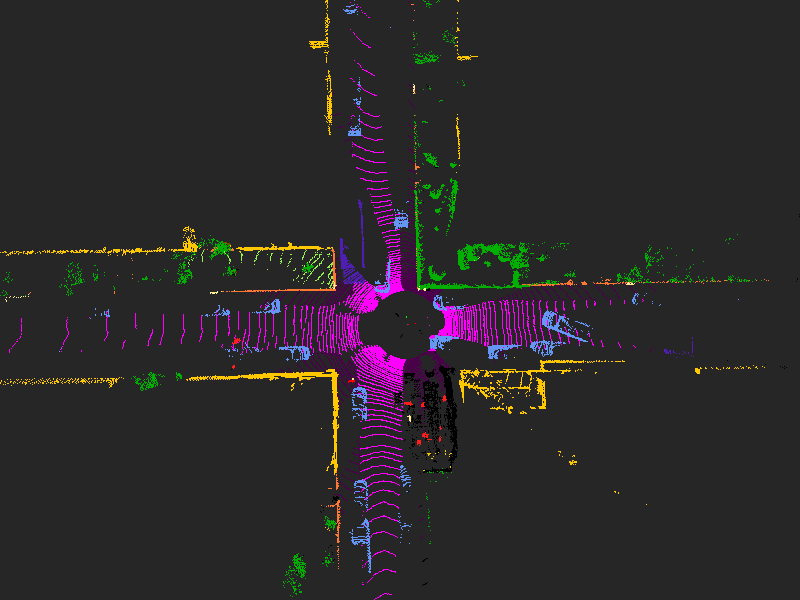
\includegraphics [width=0.5\textwidth]{figs/final-true1t.png}
        \caption {Exemplo de uma cena do SemanticKITTI com rótulos semânticos.
            (sequencia 7 - frame 993)}
    \end{figure}
\end{frame}

\begin{frame}
    \frametitle{Pré-processamento: Segmentação do Solo (GPF)}
    \begin{columns}[T]
        \begin{column}{.4\textwidth}
            \begin{block}{Objetivo}
                \vspace{0.5em}
                Identificar os pontos pertencentes ao solo.
                \vspace{0.5em}
            \end{block}
            \begin{block}<+->{Algoritmo}
                \vspace{0.5em}
                Ground Plane Fitting (GPF).
                \vspace{0.5em}
            \end{block}
        \end{column}
        \begin{column}{.6\textwidth}
            \begin{block}<+->{Como funciona}
                \begin{enumerate}[<+->]
                    \item Seleção dos pontos sementes.
                    \item Estimativa do plano: calcula o LRP, em seguida aplica
                          SVD para obter o vetor normal do plano.
                    \item Refinamento iterativo: inclui pontos próximos do plano
                          (< limiar) em iterações sucessivas, e repete o item 2.
                    \item Classificação final: pontos do solo recebem label
                          específico.
                \end{enumerate}
            \end{block}
        \end{column}
    \end{columns}
\end{frame}

\begin{frame}
    \frametitle{Pré-processamento: Clusterização de Objetos (SLR)}
    \begin{columns}[T]
        \begin{column}{.4\textwidth}
            \begin{block}{Objetivo}
                \vspace{0.5em}
                Agrupar os pontos remanescentes (não-solo) em clusters que representam objetos.
                \vspace{0.5em}
            \end{block}
            \begin{block}<+->{Algoritmo}
                \vspace{0.5em}
                Scan Line Run (SLR).
                \vspace{0.5em}
            \end{block}
        \end{column}
        \begin{column}{.6\textwidth}
            \begin{block}<+->{Como funciona}
                \begin{enumerate}[<+->]
                    \item Agrupamento inicial por scanline preservando estrutura sequencial LiDAR.
                    \item Identificação de "runs": segmentos contínuos com distância < limiar.
                    \item Propagação de rótulos entre scanlines adjacentes (< limiar).
                    \item Resolução de equivalências via tabela para fundir rótulos duplicados.
                    \item Atribuição final: cada cluster recebe identificador único.
                \end{enumerate}
            \end{block}
        \end{column}
    \end{columns}
\end{frame}


\begin{frame}
    \frametitle{Pré-processamento: Extração de Características}
    \begin{columns}[T]
        \begin{column}{.4\textwidth}
            \begin{block}{Objetivo}
                \vspace{0.5em}
                Extrair vetor de características para cada cluster gerado pelo SLR.
                \vspace{0.5em}
            \end{block}
            \begin{block}<+->{Saída}
                \vspace{0.5em}
                Vetor de 24 características + 2 rótulos por cluster.
                \vspace{0.5em}
            \end{block}
        \end{column}
        \begin{column}{.6\textwidth}
            \begin{block}<+->{Características Extraídas}
                \begin{itemize}[<+->]
                    \item Posição espacial (9 valores):
                          \begin{itemize}
                              \item Centroide (x, y, z) - posição central
                              \item Bounding box: pontos mín/máx (x, y, z)
                          \end{itemize}
                    \item Distribuição espacial (15 valores):
                          \begin{itemize}
                              \item Histogramas X, Y, Z (5 bins cada)
                              \item Capturam forma e orientação do cluster
                          \end{itemize}
                    \item Rótulos (2 valores):
                          \begin{itemize}
                              \item True label (anotação ground truth)
                              \item Predicted label (placeholder para classificação)
                          \end{itemize}
                \end{itemize}
            \end{block}
        \end{column}
    \end{columns}
\end{frame}

\begin{frame}
    \frametitle{Classificação: PointNet Modificada}
    \begin{columns}[T]
        \begin{column}{.4\textwidth}
            \begin{block}{Entrada}
                \vspace{0.5em}
                Vetores de 24 características
                \vspace{0.5em}
            \end{block}
            \begin{block}<+->{Saida}
                \vspace{0.5em}
                Clusters classificados em 20 categorias semânticas.
                \vspace{0.5em}
            \end{block}
        \end{column}
        \begin{column}{.6\textwidth}
            \begin{block}<+->{Modificações Implementadas}
                \begin{itemize}[<+->]
                    \item Expansão da capacidade:
                          \begin{itemize}
                              \item Maior largura (mais canais)
                              \item Maior profundidade (mais camadas)
                              \item compensar a redução da dimensionalidade
                              \item Redução significativa na dimensionalidade
                                    mitiga custo computacional da expansão do
                                    modelo.
                          \end{itemize}
                    \item Adaptação da entrada para aceirar as 24 características
                    \item Normalização atualizada de BatchNorm para InstanceNorm1d
                \end{itemize}
            \end{block}
        \end{column}
    \end{columns}
\end{frame}

%---------------------------------------------------------
\section{Resultados}
%---------------------------------------------------------

\setLayout{mainpoint}
\setBGColor{UFGBlue}
\begin{frame}
    \frametitle{Resultados}
\end{frame}
\setLayout{vertical}
\setBGColor{UFGBlue}

\begin{frame}
    \frametitle{Saida do GPF}
    \begin{figure}
        \centering
        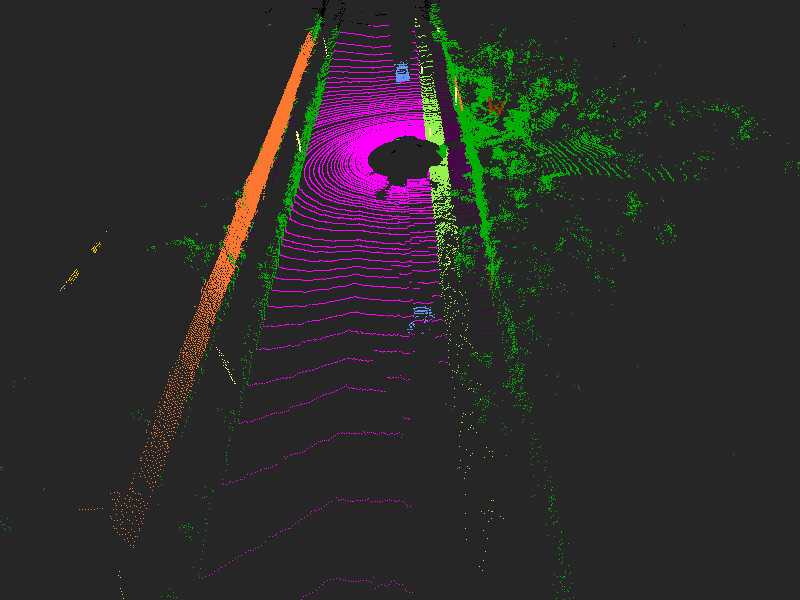
\includegraphics[width=0.48\textwidth]{figs/label_2_s4f75.png}
        \hspace{0.02\textwidth}
        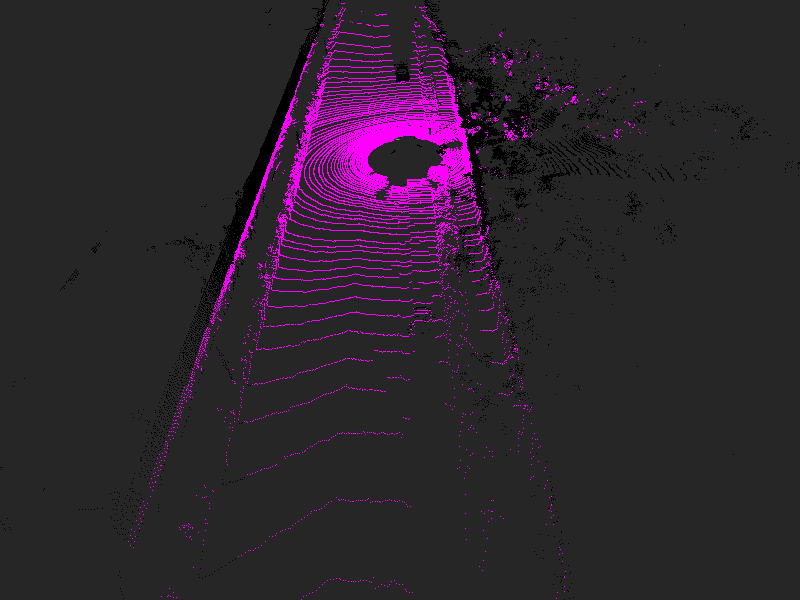
\includegraphics[width=0.48\textwidth]{figs/gpf_2_s4f75.png}
        \caption {Comparação entre rótulos reais (esquerda) segmentação predita
            pelo GPF (direita), sequencia 4 - frame 75.}
    \end{figure}
\end{frame}

\begin{frame}
    \frametitle{Saida do SLR}
    \begin{figure}
        \centering
        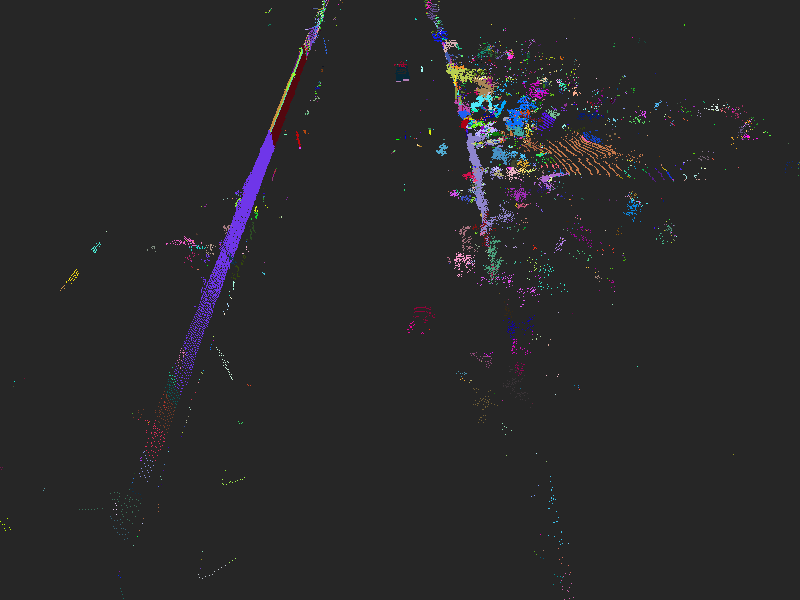
\includegraphics[width=0.48\textwidth]{figs/slr_2_s4f75.png}
        \caption {Saida do SLR, sequencia 4 - frame 75.}
    \end{figure}
\end{frame}

\begin{frame}
    \frametitle{Analise dos Clusters Inconsistentes}
    \begin{figure}
        \centering
        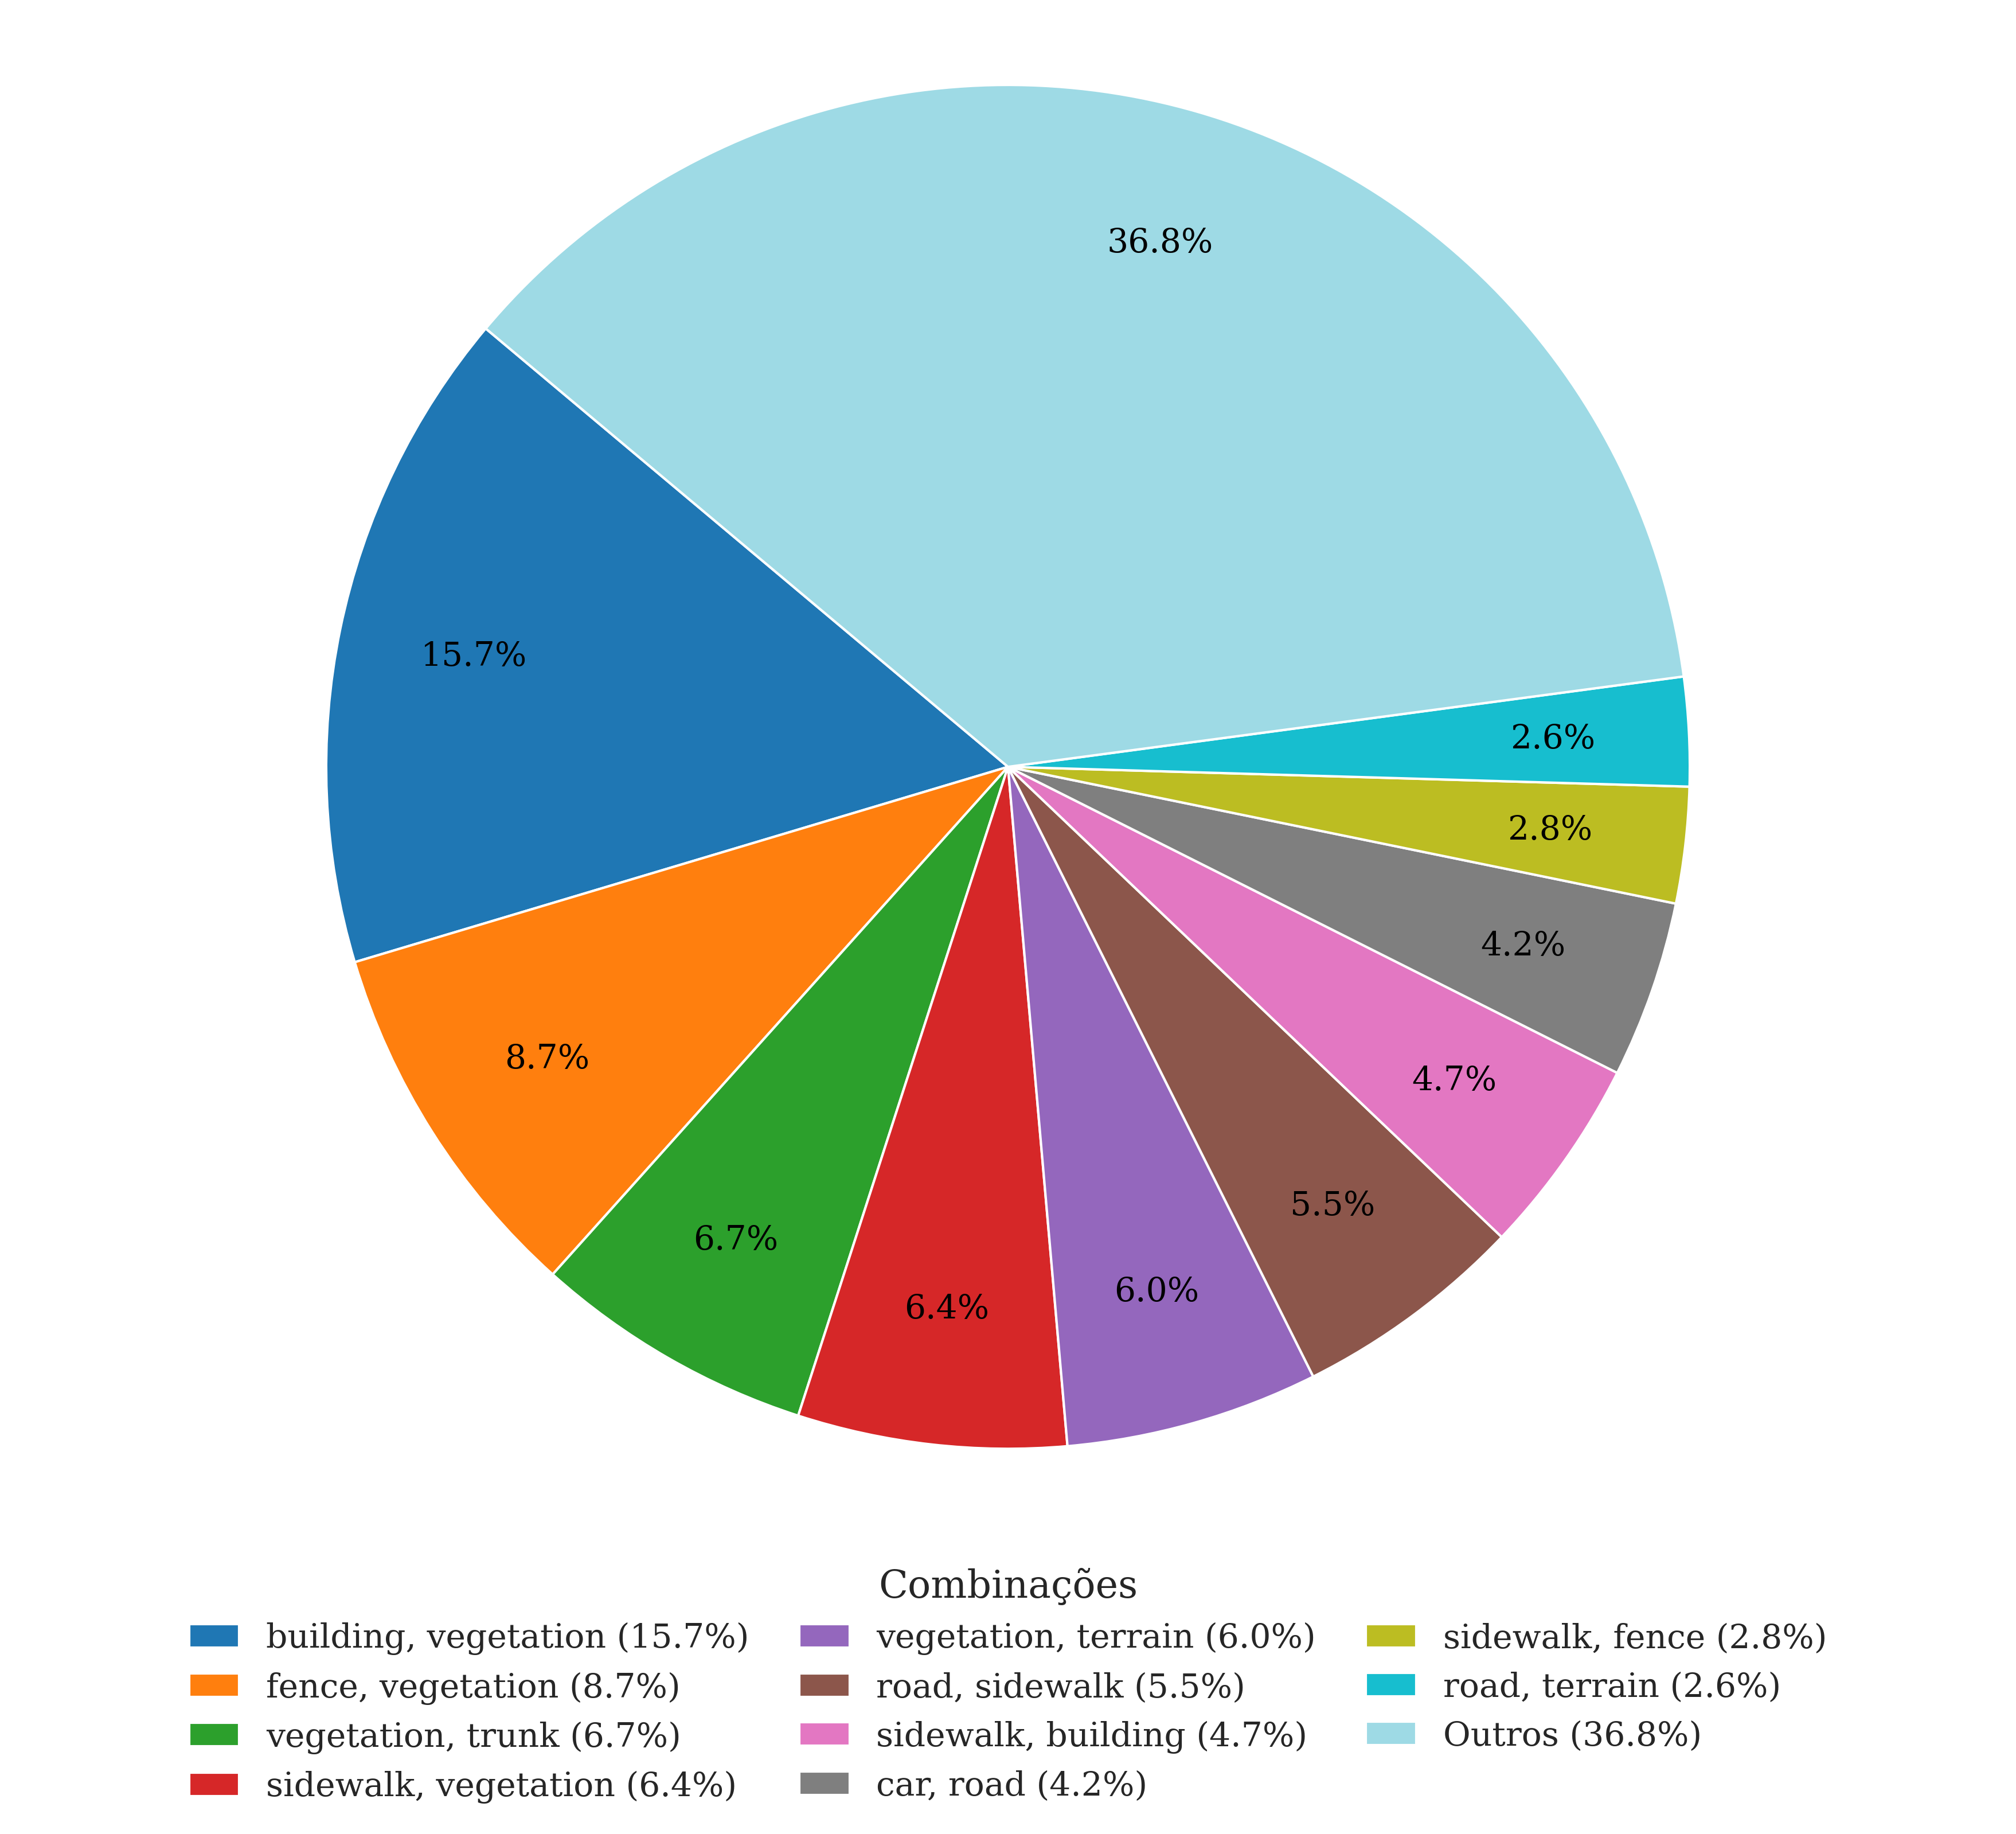
\includegraphics[width=0.48\textwidth]{figs/plot-5.png}
        \caption {Combinações mais frequentes dos clusters inconsistentes, sequencia 0.}
    \end{figure}
\end{frame}

\begin{frame}
    \frametitle{Analise dos Clusters Inconsistentes}
    \begin{figure}
        \centering
        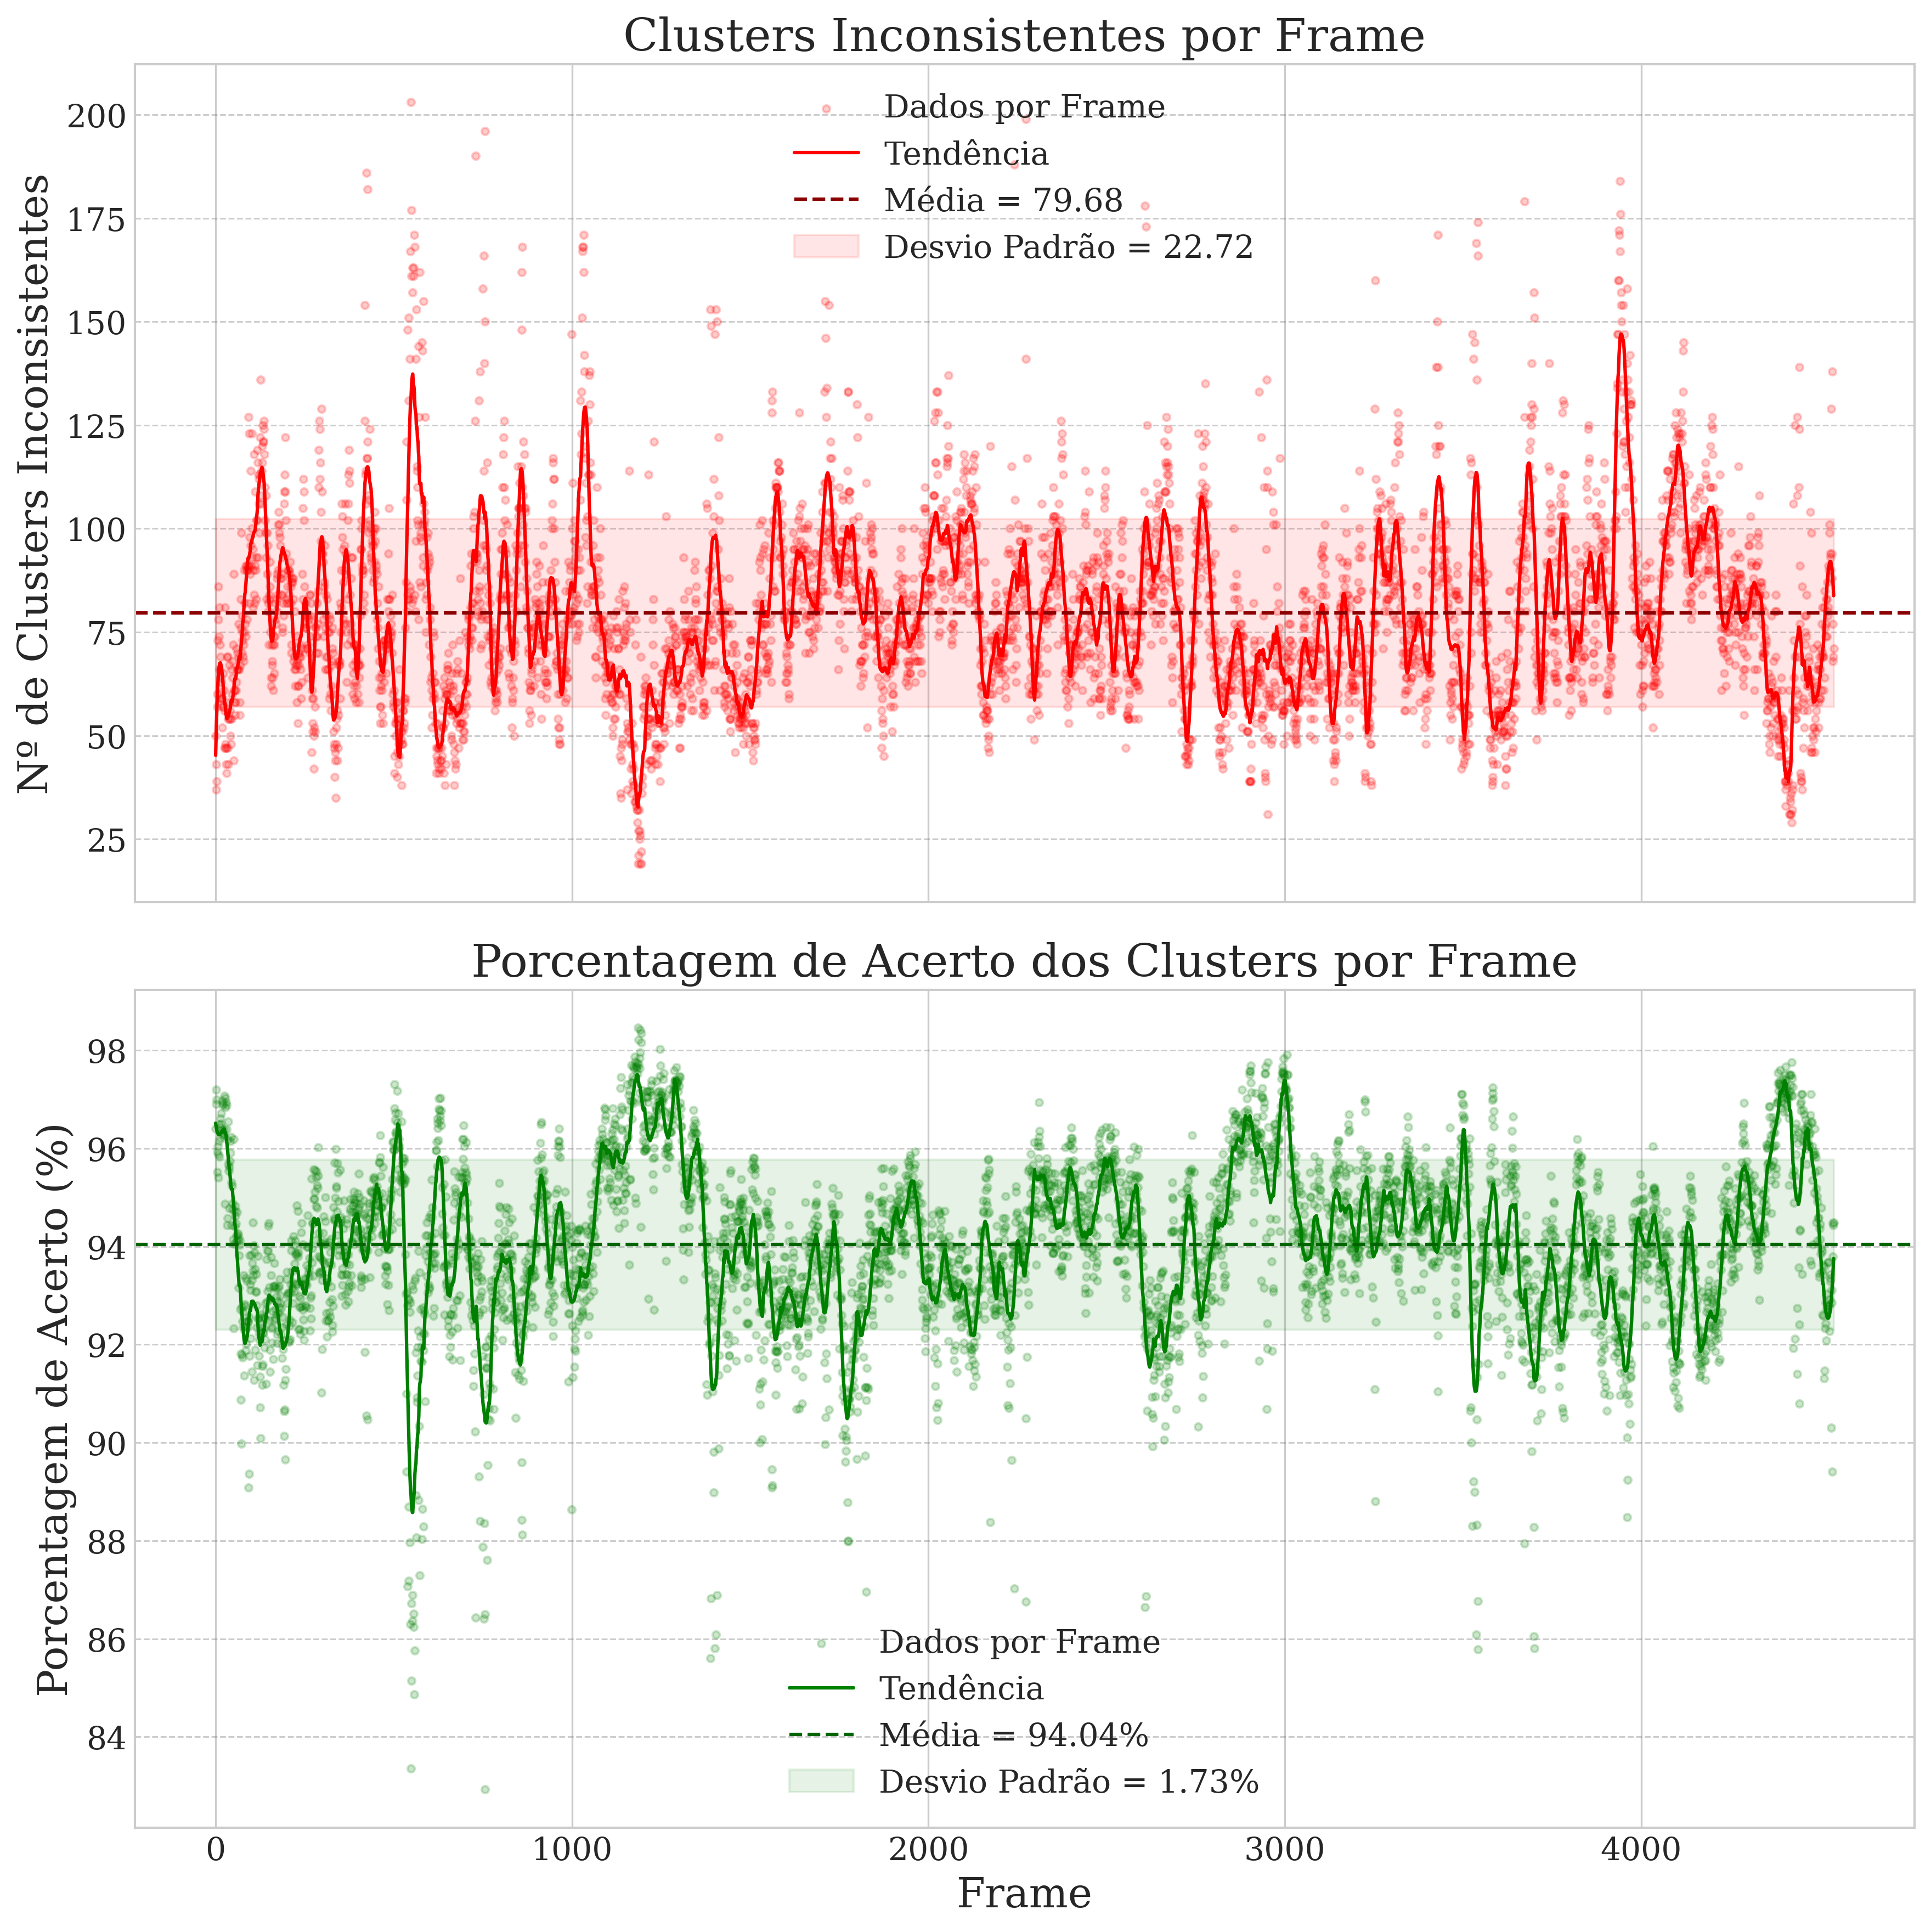
\includegraphics[width=0.48\textwidth]{figs/plot-3.png}
        \caption {Gráfico de analise dos clusters inconsistentes, sequencia 0.}
    \end{figure}
\end{frame}

\begin{frame}
    \frametitle{Clusters após Extração de Características}
    \begin{figure}
        \centering
        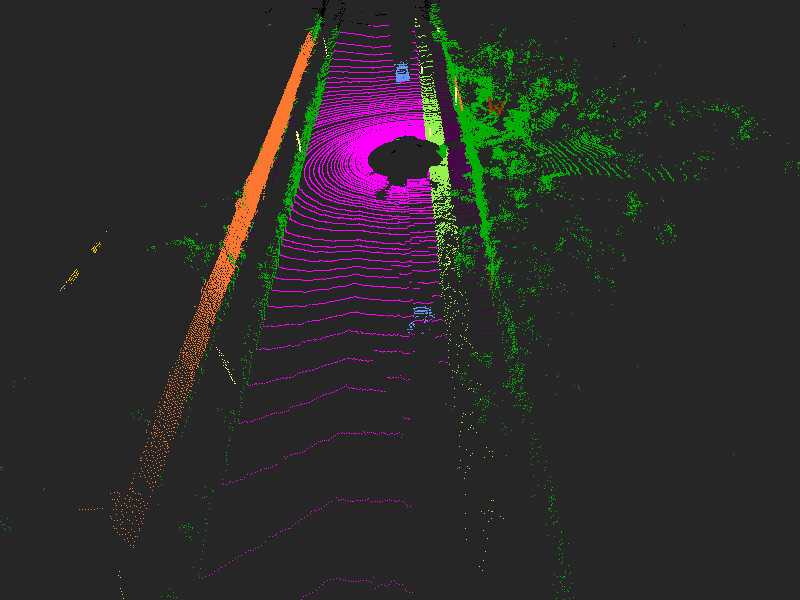
\includegraphics[width=0.48\textwidth]{figs/label_2_s4f75.png}
        \hspace{0.02\textwidth}
        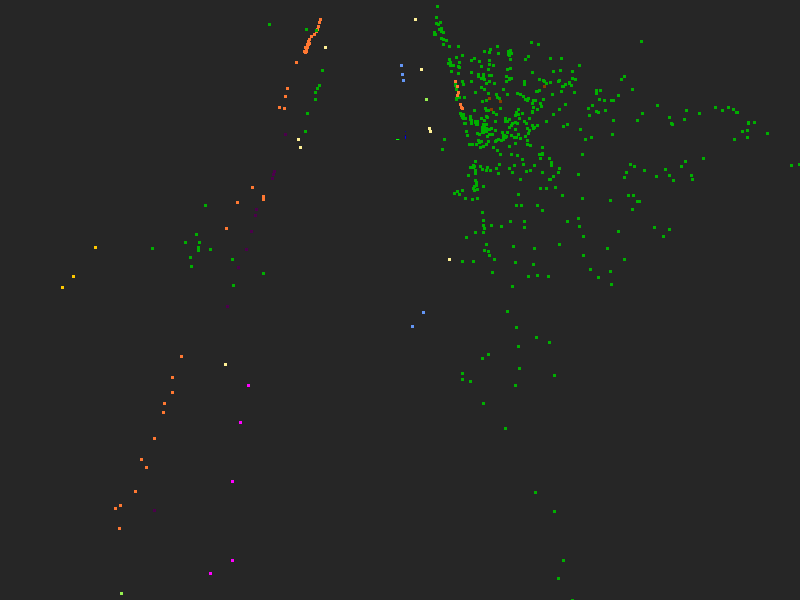
\includegraphics[width=0.48\textwidth]{figs/cluster_2_s4f75.png}
        \caption {Comparação dos dados originais (esquerda) com os clusters
            após extração de características (direita), sequencia 4 - frame 75.}
    \end{figure}
\end{frame}

\begin{frame}
    \frametitle{Avaliação da Redução de Dimensionalidade}
    \begin{figure}
        \centering
        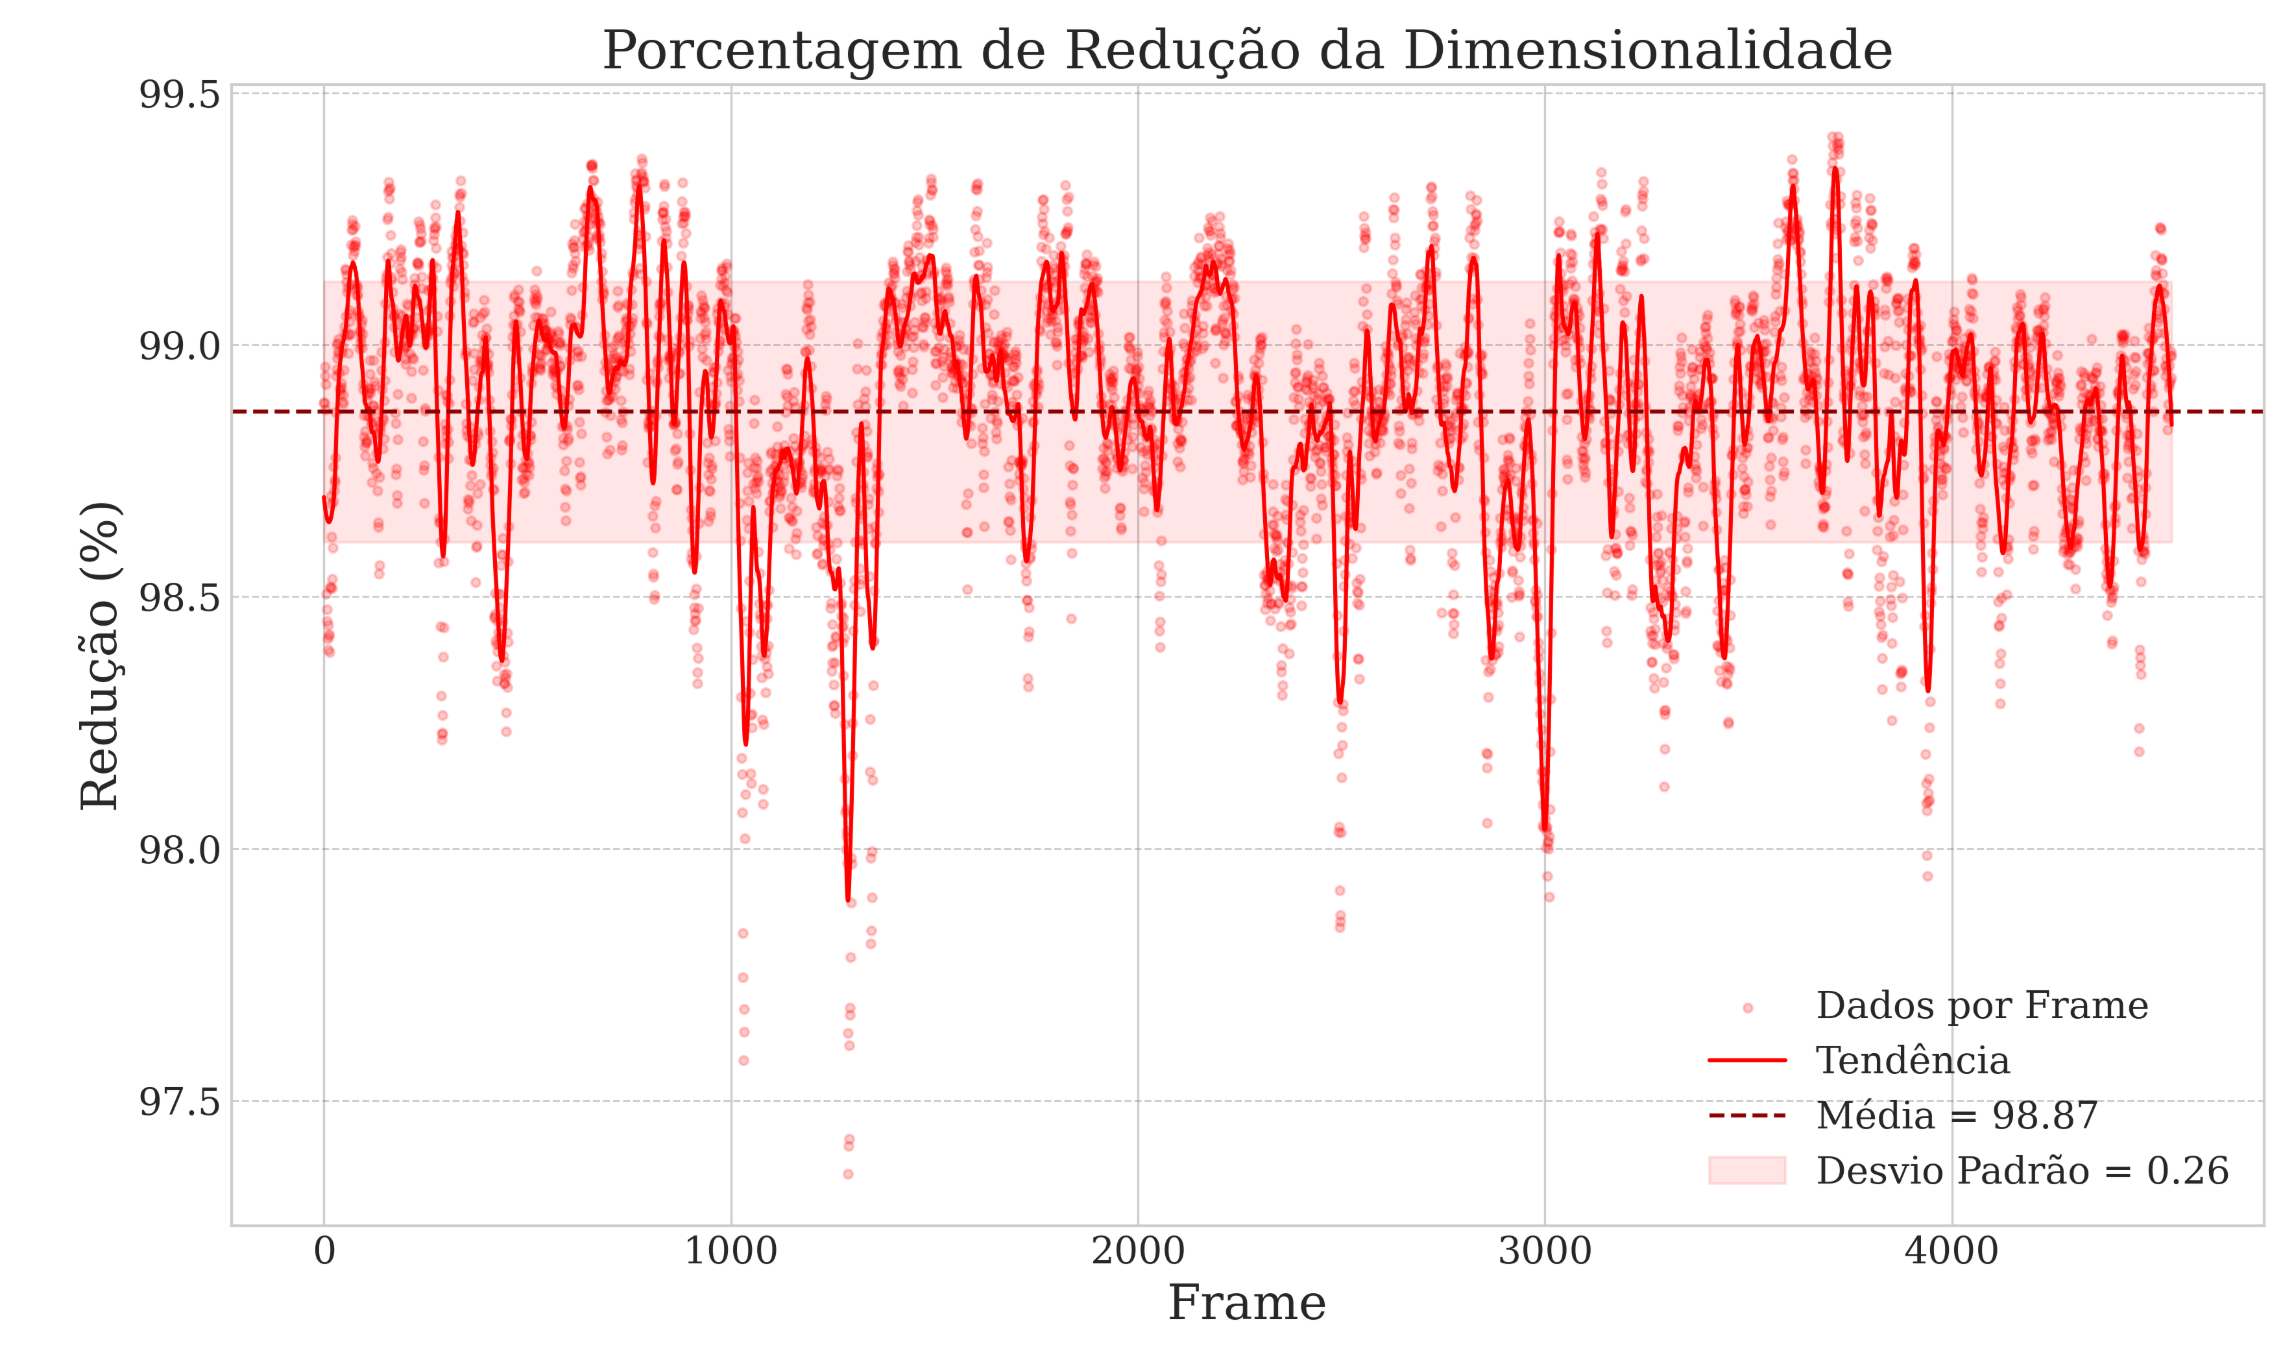
\includegraphics[width=0.75\textwidth]{figs/plot-1-2.png}
        \caption {Gráfico de analise da redução de dimensionalidade, sequencia 0.}
    \end{figure}
\end{frame}

\begin{frame}
    \frametitle{Classificação}
    \begin{figure}
        \centering
        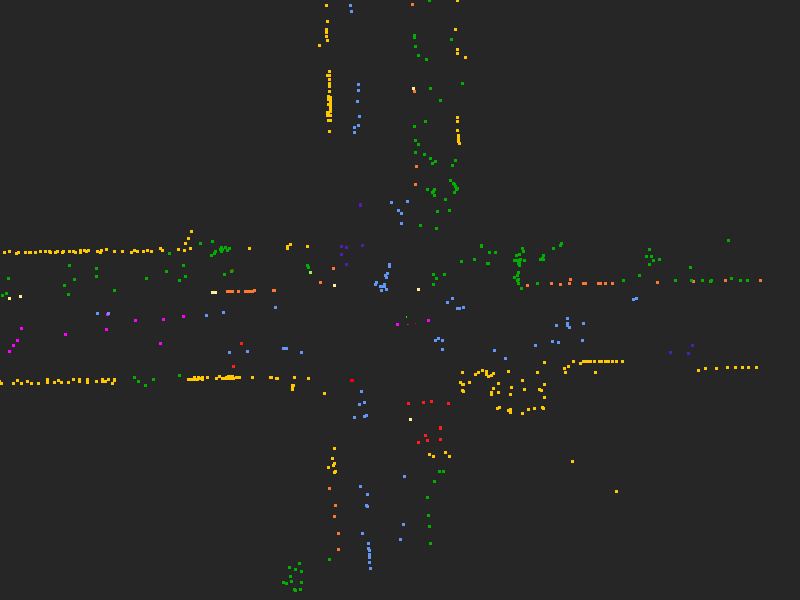
\includegraphics[width=0.48\textwidth]{figs/final-true2t.png}
        \hspace{0.02\textwidth}
        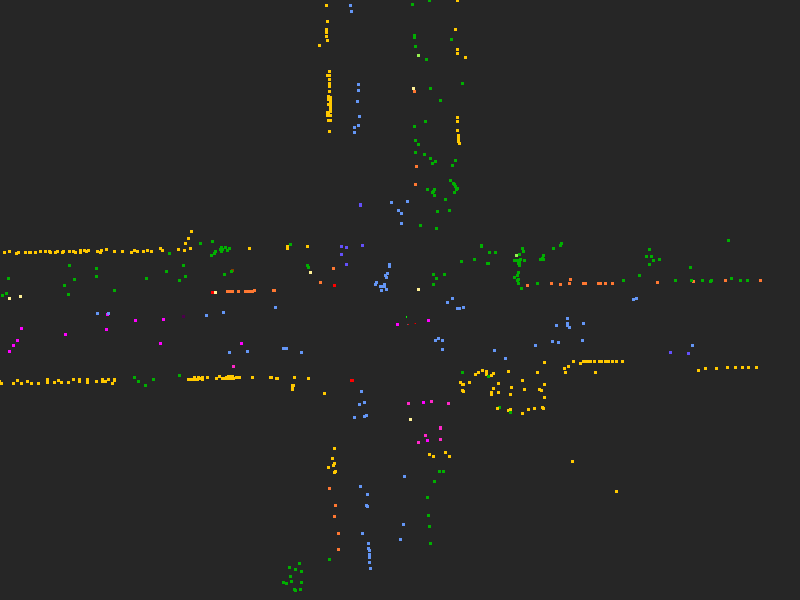
\includegraphics[width=0.48\textwidth]{figs/final-predt.png}
        \caption {Comparação entre cluster obtidos (esquerda) com a
            classificação do modelo (direita), sequencia 7 - frame 993.}
    \end{figure}
\end{frame}

\begin{frame}
    \frametitle{Desempenho do Modelo}
    \begin{figure}
        \centering
        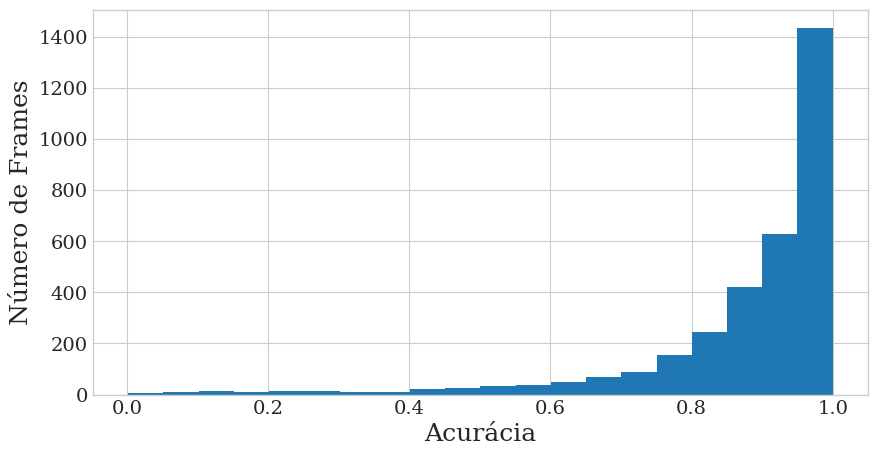
\includegraphics[width=0.75\textwidth]{figs/plot-6.png}
        \caption {Gráfico da distribuição de acu, sequencia 0.}
    \end{figure}
\end{frame}

%---------------------------------------------------------
\section{Conclusão e Trabalhos Futuros}
%---------------------------------------------------------

\setLayout{mainpoint}
\setBGColor{UFGBlue}
\begin{frame}
    \frametitle{Conclusão e Trabalhos Futuros}
\end{frame}
\setLayout{vertical}
\setBGColor{UFGBlue}

\begin{frame}
    \frametitle{Conclusões}
    \begin{itemize}
        \item<+-> O trabalho validou um pipeline híbrido que combina
              processamento geométrico clássico com aprendizado profundo para
              segmentação semântica de nuvens de pontos.
        \item<+-> Os resultados (redução de 98.8\%, acurácia de 93.3\%)
              confirmam a viabilidade da metodologia para aplicações que
              demandam eficiência.
    \end{itemize}
    \begin{alertblock}<+->{Principal Contribuição}
        Demonstração de que é possível comprimir drasticamente nuvens de pontos
        LiDAR em representações de clusters, preservando a informação semântica
        essencial para a classificação.
    \end{alertblock}
\end{frame}

\begin{frame}
    \frametitle{Limitações e Trabalhos Futuros}
    \begin{columns}[T]
        \begin{column}{.5\textwidth}
            \begin{block}<+->{Limitações}
                \begin{itemize}
                    \item<+-> \textbf{Fragmentação:} clusterização geométrica
                          pode dividir objetos complexos
                    \item<+-> \textbf{Generalização limitada:} validação
                          restrita ao SemanticKITTI
                    \item<+-> \textbf{Classes minoritárias:} desempenho
                          inferior em objetos menos representados
                    \item<+-> \textbf{Otimização:} implementação não adequada
                          para tempo real
                \end{itemize}
            \end{block}
        \end{column}
        \begin{column}{.5\textwidth}
            \begin{block}<+->{Trabalhos Futuros}
                \begin{itemize}
                    \item<+-> \textbf{Robustez:} métodos de segmentação mais
                          flexíveis e resilientes
                    \item<+-> \textbf{Enriquecimento:} incluir intensidade
                          LiDAR e contexto espacial
                    \item<+-> \textbf{Generalização:} validar em múltiplos
                          datasets e sensores
                    \item<+-> \textbf{Eficiência:} otimização para hardware
                          embarcado
                    \item<+-> \textbf{Expansão:} integrar detecção de objetos e
                          estimativa de pose
                \end{itemize}
            \end{block}
        \end{column}
    \end{columns}
\end{frame}

%---------------------------------------------------------Slide 9
\setLayout{blank}
\begin{frame}
    \centering
    \vspace{2cm}
    \textbf{\Huge Obrigado!}
    \ \\
    \textbf{\Large Duvidas ou Sugestões?}
    \ \\
    \text{\footnotesize matheus.leonel@discente.ufg.com}
    \vspace{2cm}
    \begin{figure}
        \centering
        \begin{subfigure}{0.2\textwidth}
            \centering
            
\includegraphics[height=1cm]{lib/logos/infw.png}
        \end{subfigure}%
        \qquad 
        \begin{subfigure}{0.2\textwidth}
            \centering
            
\includegraphics[height=1cm]{lib/logos/ufgw.png}
        \end{subfigure}
    \end{figure}
\end{frame}
\end{document}